\documentclass{standalone}
\usepackage{tikz}
\usepackage{pgfplots}
\pgfplotsset{compat=1.18}

% use colors from dvipsnames
\usepackage[dvipsnames]{xcolor}

\newif\ifpartial
\newif\iftotal
\newif\ifpartialORtotal

% \partialtrue
\totaltrue

\makeatletter
\ifpartial
  \partialORtotaltrue
\else
  \iftotal
    \partialORtotaltrue
  \else
    \partialORtotalfalse
  \fi
\fi
\makeatother

\begin{document}
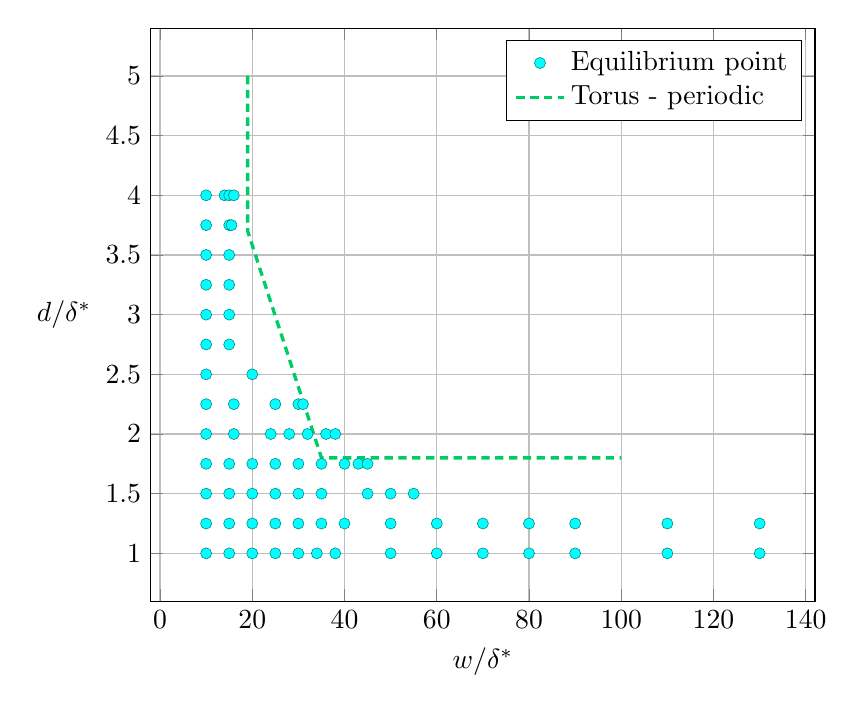
\begin{tikzpicture}
	\begin{axis}[
			xlabel={$w/\delta^*$},
			ylabel={$d/\delta^*$},
			grid=both,
			% axis lines=middle,
			ytick distance=0.5,
			ylabel style={rotate=-90, at={(-0.075,0.5)}},
			legend style={
					legend cell align=left,
				},
			scale only axis,
		]
		\def\colorA{Cyan}
		\def\colorB{YellowOrange}
		\def\colorC{gray!80!black}
		\def\colorD{SpringGreen}
		\def\size{2pt}
		\def\thickness{very thin}
		\def\thicknessline{very thick}
		\def\linestyle{densely dashed}
		\def\mark{*}

		% Each point has x y and a color
		\addplot[
			mark=\mark,
			only marks,
			mark size=\size,
			draw=\colorA!50!black,
			\thickness,
			fill=\colorA,
		] coordinates {
    (10.0, 1.0)
    (15.0, 1.0)
    (20.0, 1.0)
    (25.0, 1.0)
    (30.0, 1.0)
    (34.0, 1.0)
    (38.0, 1.0)
    (50.0, 1.0)
    (60.0, 1.0)
    (70.0, 1.0)
    (80.0, 1.0)
    (90.0, 1.0)
    (110.0, 1.0)
    (130.0, 1.0)
    (10.0, 1.25)
    (15.0, 1.25)
    (20.0, 1.25)
    (25.0, 1.25)
    (30.0, 1.25)
    (35.0, 1.25)
    (40.0, 1.25)
    (50.0, 1.25)
    (60.0, 1.25)
    (70.0, 1.25)
    (80.0, 1.25)
    (90.0, 1.25)
    (110.0, 1.25)
    (130.0, 1.25)
    (10.0, 1.5)
    (15.0, 1.5)
    (20.0, 1.5)
    (25.0, 1.5)
    (30.0, 1.5)
    (35.0, 1.5)
    (45.0, 1.5)
    (50.0, 1.5)
    (55.0, 1.5)
    (10.0, 1.75)
    (15.0, 1.75)
    (20.0, 1.75)
    (25.0, 1.75)
    (30.0, 1.75)
    (35.0, 1.75)
    (40.0, 1.75)
    (43.0, 1.75)
    (45.0, 1.75)
    (10.0, 2.0)
    (16.0, 2.0)
    (24.0, 2.0)
    (28.0, 2.0)
    (32.0, 2.0)
    (36.0, 2.0)
    (38.0, 2.0)
    (10.0, 2.25)
    (16.0, 2.25)
    (25.0, 2.25)
    (30.0, 2.25)
    (31.0, 2.25)
    (10.0, 2.5)
    (20.0, 2.5)
    (10.0, 2.75)
    (15.0, 2.75)
    (10.0, 3.0)
    (15.0, 3.0)
    (10.0, 3.25)
    (15.0, 3.25)
    (10.0, 3.5)
    (15.0, 3.5)
    (10.0, 3.75)
    (15.0, 3.75)
    (15.5, 3.75)
    (10.0, 4.0)
    (14.0, 4.0)
    (15.0, 4.0)
    (16.0, 4.0)
		};
		\iftotal
			\addplot[
				mark=\mark,
				only marks,
				mark size=\size,
				draw=\colorB!50!black,
				\thickness,
				fill=\colorB,
			] coordinates {
    (58.0, 1.5)
    (47.0, 1.75)
    (50.0, 1.75)
    (53.0, 1.75)
    (55.0, 1.75)
    (40.0, 2.0)
    (42.0, 2.0)
    (44.0, 2.0)
    (46.0, 2.0)
    (48.0, 2.0)
    (50.0, 2.0)
    (51.0, 2.0)
    (32.0, 2.25)
    (33.0, 2.25)
    (35.0, 2.25)
    (40.0, 2.25)
    (43.0, 2.25)
		};
		\fi

		\ifpartialORtotal
			\addplot[
				mark=\mark,
				only marks,
				mark size=\size,
				draw=\colorC!50!black,
				\thickness,
				fill=\colorC,
			] coordinates {
    (60.0, 1.5)
    (65.0, 1.5)
    (70.0, 1.5)
    (75.0, 1.5)
    (80.0, 1.5)
    (100.0, 1.5)
    (120.0, 1.5)
    (57.0, 1.75)
    (60.0, 1.75)
    (70.0, 1.75)
    (90.0, 1.75)
    (110.0, 1.75)
    (130.0, 1.75)
    (52.0, 2.0)
    (53.0, 2.0)
    (54.0, 2.0)
    (56.0, 2.0)
    (58.0, 2.0)
    (60.0, 2.0)
    (65.0, 2.0)
    (70.0, 2.0)
    (80.0, 2.0)
    (45.0, 2.25)
    (47.0, 2.25)
    (50.0, 2.25)
    (55.0, 2.25)
    (60.0, 2.25)
    (21.0, 2.5)
    (22.0, 2.5)
    (23.0, 2.5)
    (24.0, 2.5)
    (25.0, 2.5)
    (30.0, 2.5)
    (35.0, 2.5)
    (40.0, 2.5)
    (45.0, 2.5)
    (15.5, 2.75)
    (16.0, 2.75)
    (16.5, 2.75)
    (17.0, 2.75)
    (18.0, 2.75)
    (19.0, 2.75)
    (20.0, 2.75)
    (15.5, 3.0)
    (16.0, 3.0)
    (17.0, 3.0)
    (18.0, 3.0)
    (22.0, 3.0)
    (26.0, 3.0)
    (15.5, 3.25)
    (16.0, 3.25)
    (16.5, 3.25)
    (15.5, 3.5)
    (16.0, 3.5)
    (16.0, 3.75)
    (16.5, 3.75)
    (16.5, 4.0)
    (17.0, 4.0)
    (18.0, 4.0)
    (19.0, 4.0)
		};
		\fi

		% %%%%%% Lines
		\iftotal
			\addplot[
				smooth,
				no marks,
				draw=\colorB!70!black,
				\thicknessline,
				\linestyle,
			] coordinates {
    (31.5, 2.25)
    (39.0, 2.0)
    (46.0, 1.75)
    (56.5, 1.5)
		};
		\fi

		\ifpartialORtotal
			\addplot[
				smooth,
				no marks,
				draw=\colorC!50!black,
				\thicknessline,
				\linestyle,
			] coordinates {
    (16.25, 4.0)
    (15.75, 3.75)
    (15.25, 3.5)
    (15.25, 3.25)
    (15.25, 3.0)
    (15.25, 2.75)
    (20.5, 2.5)
		};

			\addplot[
				smooth,
				no marks,
				draw=\colorC!50!black,
				\thicknessline,
				\linestyle,
			] coordinates {
    (44.0, 2.25)
    (51.5, 2.0)
    (56.0, 1.75)
    (59.0, 1.5)
    (65.0, 1.375)
    (70.0, 1.375)
    (75.0, 1.375)
    (80.0, 1.375)
    (100.0, 1.375)
    (120.0, 1.375)
    (130.0, 1.375)
		};
		\fi

		\addplot[
			draw,
			no marks,
			draw=\colorD!80!black,
			\thicknessline,
			\linestyle,
		] coordinates {
    (19.0, 5.0)
    (19.0, 3.7)
    (35.0, 1.8)
    (100.0, 1.8)
		};

		\ifpartial
			\legend{
				{Equilibrium point},
				% {Torus - periodic},
				{Chaos},
				% {Hopf bifurcation},
				{Breakdown},,
				{Experimental data},
			}
		\else
			\legend{
				{Equilibrium point},
				{Torus - periodic},
				{Chaos},
				{Hopf bifurcation},
				{Breakdown},,
				{Experimental data},
			}
		\fi

	\end{axis}
\end{tikzpicture}
\end{document}
